\begin{figure}
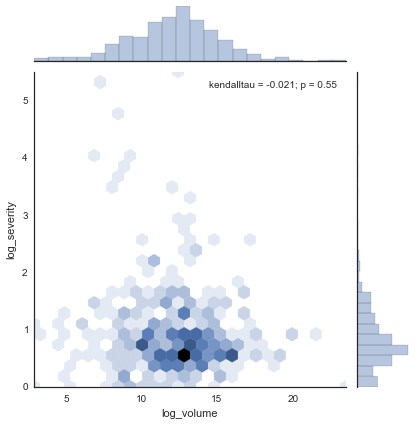
\includegraphics[width=\columnwidth]{severity_volume}
\caption{\textcolor{red}{Not sure this figure is needed. What information does it convey?}}
\end{figure}
Our daily price and volume data are scraped from \url{http://coinmarketcap.com}, which is the most exhaustive data source on all cryptocoins \footnote{\textcolor{red}{For robustness analysis smaller subsets of the coins where available from coin}}.
%JULIAN: Didn't follow the above footnote
The site contains the historical data for 660 cryptocoins, each starting at the earliest date the coin appeared in an exchange. We were able to match \textcolor{red}{376} (out of 679) coins to their introducers in the forums. The price and volume data are aggregated over 77 exchanges which span across several countries. Nevertheless, only a few exchanges such as Bitfinex, BTC-E, Poloniex and Cryptsy carry the bulk of the market volume.
